\subsection{Flood map}
The flood map was obtained by processing Sentinel-1 GRD data with the UN-SPIDER change detection method in the GEE tool. Prior to processing, four dates are provided for a collection of pre- and post-flood images(Tab.\ref{tab:collectionofimage}. From these dates, the GEE searches for available images according to the parameters namely the region of interest, the polarisation and the satellite ascending pass. In our case of the flood study of August  8\textsuperscript{th}, 2020 in Douala, two images S1 of 2020-08-02 were used as the pre-flood and S1 2020-08-26 as the post-flood(Fig. \ref{fig:pre_post_flood}. We have privileged a common DESCENDING pass to avoid different geometric distortion due to the angle.
\begin{table}[hbt!]\centering
\caption{Four dates defining a collection of images before and after the flood}
\begin{tabular}{lll}
\hline
\textbf{}       & \textbf{Start} & \textbf{End} \\
\hline
\textbf{Before} & 2020-08-01     & 2020-08-19   \\
\textbf{After}  & 2020-08-21     & 2020-09-01  \\
\hline
\end{tabular}\label{tab:collectionofimage}
\end{table}

\begin{figure*} %[hbt!]
	\centering
	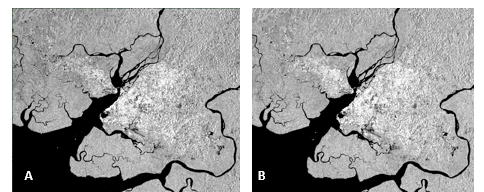
\includegraphics[width=5in]{figure/changedetection.png}
	\caption{Sentinel-1 image of VH available for the flood study of August  8\textsuperscript{th}, 2020 in Douala. The two images S1 of 2020-08-02(A) were used as the pre-flood and S1 2020-08-26(B) as the post-flood}
	\label{fig:pre_post_flood}
\end{figure*}

The UN-SPIDER method processing includes a default difference threshold value of 1.25. Unlike conventional methods, this value is applied to the difference image (after flooding - before flooding) and not to each individual image\ref{fig:flood_maps}. In our case, this default value allowed for more efficient results by preventing flood extent from having many false positive or negative signals. 


\begin{figure*}[hbt!]
	\centering
	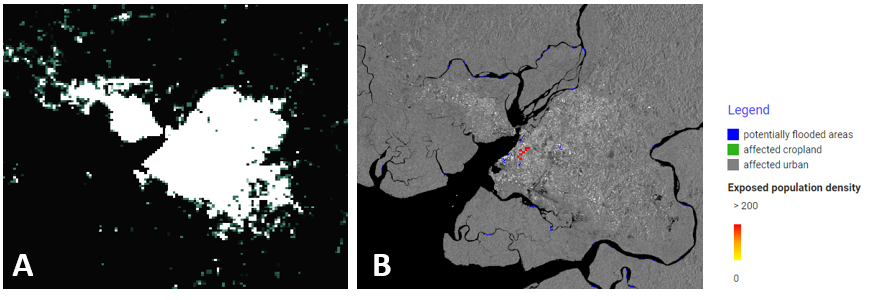
\includegraphics[width=0.8\linewidth]{figure/vh2020.png}
	\caption{UN-SPIDER change detection approach\cite{un-spider}. A: Population density layer where bright pixels shows denser populated areas. B: Population density exposed to the flood event (from yellow-red). Flood status between: 2020-08-21 and 2020-09-15, DESCENDING, polarization = "VH", Estimated flood extent: based on Sentinel-1 imagery from 2020-08-26 to 2020-09-07, 43 hectares, Estimated number of exposed people:
based on GHSL 2015 (250m): 10900.}
	\label{fig:flood_maps}
\end{figure*}

The inundation map using VH polarization results are presented in the figure \ref{fig:flood_maps}. Given the nature of the study area, such as the tightly packed buildings, distinguishing between flooded and non-flooded areas was not a straightforward task. In our case, the use of VV polarization accentuated the false classifications.
\subsection{Discussion}
The location of Douala at the south-eastern shore of the Wouri River estuary makes it particularly susceptible to flooding
which could be exacerbated by storm surges and sea level rise. The river
channel is flanked on either side by densely populated communities.

Areas of concern are communities such as Bonaberi and Deido which are
located close to a constriction around the Bonaberi/Wouri bridge along
the channel of the Wouri River. Such constrictions could arise when
confining margins occur on both sides of a channel at the same reach
\cite{EnvironmentAgency2021}. Channel constrictions could instigate
high velocity river flows which can rapidly diffuse into the surrounding
flood plains and communities. Another implication is the possible
expansion of the floodplain in areas downstream of the constriction such
as in Bonanjo. 

High population density also increases vulnerability.  According to our estimates, the central areas were more exposed over a flood extent of 43 hectares with an estimated number of exposed people based on the 2015 GHSL (250m) of 10,900 people.
These data are based however on the threshold estimation parameter. As for the tool developed by UN SPIDER, the results can produce information used in particular by correlating them with soil data to estimate the financial damage caused by a flood.








